\section{RationalGRL: Logical Framework}
\label{sect:formalframework}

In Section~\ref{sect:gmas} we developed a list of critical questions and argument schemes by analyzing transcripts of discussions about the development of a traffic simulator. The resulting list is shown in Table~\ref{table:argument-schemes}. We then presented the RationalGRL framework in secton~\ref{sect:overview}, consisting of a modeling language, a metamodel, and various examples of using the argument schemes and critical questions. In section~\ref{sect:meth+tool} we explained how this framework can be used by practitioners by explaining the methodology and tool support.

In this section we present a formalization of RationalGRL based on formal logic. This is done for multiple reasons: (i) Most approaches in formal argumentation use formal logic, allowing us to employ existing technique directly in order to compute which arguments are accepted and which are rejected, (ii) we can be more precise about how critical questions are answered, (iii) we can show that RationalGRL models can be translated in to valid GRL models and visa versa in a precise way, and (iv) the formal approach is a basis for automating the framework in terms of tool support.

In the first two subsections we formalize a static representation of our framework: We provide a formal specification of a GRL model based on the GRL metamodel (Section \ref{sect:metamodel}) in the first subsection, and we extend this with arguments and attack links in the second subsection, hereby obtaining a formal specification of a RationalGRL model. 

In the third subsection we develop algorithms in order to translate a GRL model into a RationalGRL model, and visa versa.

In the fourth and final subsection we turn to the dynamics of our framework. We develop algorithms for instantiating argument schemes and for answering critical questions. 

\subsection{Formal Specification of GRL}
\label{sect:formalframework:grl}

In this subsection we formalize a GRL model based on the GRL metamodel and the jUCMNav implementation. We first formalize elements of GRL (intentional elements and actors), and then formalize the links.

\subsubsection{Intentional Element, beliefs and actors}

We start with some general definition that we use in subsequent definitions.

\begin{definition}[General definitions]
\label{def:set-definitions}
Throughout this section, we adopt the convention that variables start with a lowercase letter (e.g, $id, i, j, name, ie, goal$), and sets and constants start with an uppercase letter (e.g., $Type, AND, Goal$).

We define the following sets:
\begin{itemize}
\item $IETypes = \{Softgoal, Goal, Task, Resource\}$,
\item $Types = IETypes \cup \{Actor, Contr, Dep,$\\ \qquad $Decomp, Belief, GenArg\}$
\item $Names$ is a finite set of strings.
\item $DecompTypes = \{AND,OR,XOR\}$.
\item $ContribValues = \{Break, Hurt, Some\ nega-$ $tive, Unknown, Some\  positive, Help, Make\},$
\end{itemize}
\end{definition}

Next we define an intentional element.

\begin{definition}[Intentional Element]
\label{def:ie}
An intentional element $ie\in \mathbb{N}\times IETypes\times Names\times DecompType$ is a relation, where $ie = (id, type, name, decomptype)$ means:
\begin{itemize}
\item $id\in \mathbb{N}$ is a unique identifier for the element,
\item $type\in IETypes$ specifies the type of the element,
\item $name \in Names$ is a string description of the element,
\item $decomptype\in DecompType$ refers to the type of decomposition.\footnote{Note that the decomposition type is relevant only if the element is in fact decomposed into other elements, but since the jUCMNav implementation defines the decomposition type on the element, we do the same here.}
\end{itemize}
A set of intentional elements is denoted by $IE$.
\end{definition}

The definition above is sufficient to capture all intentional elements used in GRL. However, we present some syntactic sugar in the next definition by abbreviating the definition above in various ways. This does not add anything new to the previous definition, but it simplifies some of the notation.

\begin{definition}[Notation]
\label{def:notation}
We adopt three conventions simplifying our notation:
\begin{itemize}
\item
We refer to the element of a tuple using the dot (".") notation. That is, we may for instance refer to the id, type, name and decomposition type of an $IE$ with respectively $ie.id$, $ie.type$, $ie.name$, and $ie.decomptype$.
\item 
We refer to a set of elements with the same id $i$  using the $i$ subscript on the set. For instance a set of IEs with id $i$ is denoted by $IE_i$, and if this is a single element, we denote it by $ie_i$\footnote{In GRL, there always exists at most one element for every id (see Def.~\ref{def:grl-model}), in RationalGRL, however, this condition does not hold (see Def.~\ref{def:rationalgrl-model}).} For instance, we may refer to the intentional element $ie = (0, Goal, \text{Make profit}, AND)$ with $ie_0$ and write $ie_0.type = Goal$, $ie_0.name = \text{Make profit}$, and $ie_0.decompositiontype = AND$. 
\item
We can also refer to intention elements of a specific type simply by $type_{id}$. For instance, we can abbreviate the element in the previous item with $goal_0$ and write $goal_0.name = \text{Make profit}$, and $goal_0.decomptype = AND$.
\end{itemize}
\end{definition}

\paragraph{Rationale and example} Throughout this section we use the example in Figure~\ref{fig:example-small}, which is shown in Figure~\ref{fig:example-small2} as well. Our formalization of GRL is very much in line with the way in which GRL models are represented in the open-source Eclipse-based tool jUCMNav.\footnote{See \url{http://jucmnav.softwareengineering.ca/foswiki/ProjetSEG}} This tool is actively developed and has a rich number of features for the analysis of both GRL and URN models. By keeping our formalization in line with this tool, we simplify the translation step from models in the RationalGRL tool to models in the jUCMNav tool.

Some of the IEs in Figure~\ref{fig:example-small2} can be formalized using Def.~\ref{def:ie} as follows:
\begin{itemize}
\item $(2, goal, \text{Generate traffic}, XOR)$: This represents the goal ``Generate traffic'', which is XOR-decomposed. Note the identifier ``2'' is not shown in the GRL model, but it is stored internally.
\item $(5, resource, \text{Car objects}, AND)$: Although this element does not decompose into any other elements, it still contains an AND-decomposition. Our motivation for this choice is that it simplifies the formalization of decomposition links. It is in line with with GRL metamodel and the jUCMNav implementation.
\end{itemize}

Using the short-hand notation defined in Def.~\ref{def:notation}, we can make the following statements:
\begin{itemize}
\item $goal_2.name = \text{Generate traffic}$
\item $goal_2.decomptype = XOR$
\item $resource_5.name = \text{Car objects}$
\end{itemize}

\begin{figure}[ht]
\centering
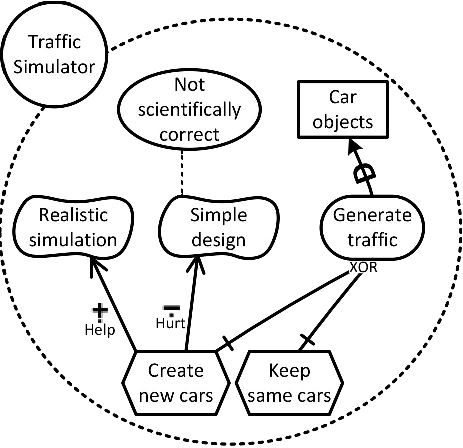
\includegraphics[width=\columnwidth]{img/Example1-new.pdf}
\caption{Example GRL model (reprint of Fig.~\ref{fig:example-small})}
\label{fig:example-small2}
\end{figure} 

\begin{definition}[Belief]
\label{def:belief}
A belief $bel\in \mathbb{N}\times Names$ is a relation where $bel=(id,name)$ means:
\begin{itemize}
\item $id\in\mathbb{N}$ is the identifier of the belief,
\item $name\in Names$ is a string description of the belief.
\end{itemize}
\end{definition}

\paragraph{Rational and example} Beliefs are different from IEs in the sense that they are not being used in decompositions, dependencies, or contributions. They merely provide additional explanation for an element. The only belief in Figure~\ref{fig:example-small2} is formalized as $(1, \text{Not scientifically correct})$.

\begin{definition}[Actor]
\label{def:actor}
An actor $act \in \mathbb{N}\times Names$ is a relation where $act=(id,name)$ means:
\begin{itemize}
\item $id\in\mathbb{N}$ is the identifier of the actor, 
\item $name\in Names$ is a string description of its name.
\end{itemize}

Similar to intentional elements, we may refer to $act = (id,name)$ with $act_{id}$ and write $act_{id}.name$ to refer to its name.

A set of actors is denoted by $Act$.
\end{definition}

\paragraph{Rationale and example} An actor is simply a pair consisting of its identifier and its name. The relation between actors and their intentional element is formalized in the next definition. 

We can formalize the actor of Figure~\ref{fig:example-small2} as $act=(0,\text{Traffic Simulator})$, and we can for instance state $act_0.name = \text{Traffic Simulator}$.

\begin{definition}[Actor-IE Relations]
\label{def:act-ie-relation}
An \emph{Actor-IE relation} $r_{ActIE}\in\mathbb{N}\times\mathbb{N}$ is a relation $(i,j)$ meaning that an actor with id $i$ has intentional element with id $j$.

A set of Actor-IE relations is denoted by $R_{ActIE}$.
\end{definition}

\paragraph{Rationale and example} The previous definition specifies relations between actors and intentional elements. Each actor can own one or multiple intentional elements, but each intentional element can only be owned by at most one actor (we will make these assumptions explicit in Def.~\ref{def:valid-grl-model}).

In Figure~\ref{fig:example-small2}, recall we formalized two IEs and the actor as follows:
\begin{itemize}
\item $(2, goal, \text{Generate traffic}, XOR)$
\item $(5, resource, \text{Car objects}, AND)$
\item $(0, \text{Traffic Simulator})$
\end{itemize}

We can then formalize the Actor-IE relationships for these elements as: $(0,2)$ and $(0,5)$.

\subsubsection{Links}

At this point we have defined all intentional elements in GRL and a containment relation between actors and intentional elements. We now turn to the GRL links.

\begin{definition}[Belief link]
\label{def:link:belief}
A \emph{belief} link: $bellink\in \mathbb{N}\times\mathbb{N}\times\mathbb{N}$ is a relation such that $bellink = (i,j)$ means
\begin{itemize}
\item $i\in \mathbb{N}$ is the unique identifier of the belief element,
\item $j\in \mathbb{N}$ is the unique identifier of the IE.
\end{itemize}
Intuitively, $bellink = (i,j)$ means that $bel_i$ is a belief for $ie_j$.

A set of belief links is denoted by $Bellink$.
\end{definition}

\paragraph{Rationale and example} The belief links can only be used to connect a belief with an intentional element, and they are not used in any of the algorithms. Instead, they can be understood as metadata, they provide additional documentation on the rationale for making certain design choices. Therefore, belief links do not require unique identifiers.

The fact that belief links only connect beliefs with IEs is not made explicit in the definition above. We make this assumption, together with various assumption, explicit in the definition of a \emph{valid GRL model} (Def.~\ref{def:valid-grl-model}). Figure~\ref{fig:example-small2} contains one belief links. It connects the following two elements:
\begin{itemize}
\item $(1, \text{Not scientifically correct})$,
\item $(4, softgoal, \text{Simple design}, AND)$.
\end{itemize}
The belief link is then formalized as $(1, 4)$.

\begin{definition}[Contribution Link]
\label{def:link:contrib}
A \emph{contribution} link: $contrib\in \mathbb{N}\times\mathbb{N}\times\mathbb{N}\times Contribvalues$ is a relation such that $contrib = (i,j,k,value)$ means
\begin{itemize}
\item $i\in \mathbb{N}$ is the unique identifier of the link,
\item $j\in \mathbb{N}$ is the unique identifier of the IE from which the contribution originates,
\item $k\in \mathbb{N}$ is the unique identifier of the IE to which is contributed.
\item $value\in ContribValues$ is the strength of the contribution.
\end{itemize}
Intuitively, $contrib = (i,j,k,value)$ means that $ie_i$ contributes to $ie_j$ with $value$.

A set of contribution links is denoted by $Contrib$.
\end{definition}

\paragraph{Rationale and example} Similar to IEs, links have identifiers as well. In Fig.~\ref{fig:example-small2}, there are two contribution links. First, let us formalize the related IEs:
\begin{itemize}
\item $(3, softgoal, \text{Realisitc simulation}, AND)$
\item $(4, softgoal, \text{Simple design}, AND)$
\item $(6, task, \text{Create new cars}, AND)$
\end{itemize}

We can formalize the contribution links as $(9, 6, 3, \text{Help})$ and $(10, 6, 4, \text{Hurt})$.

\begin{definition}[Decomposition Link]
\label{def:link:decomp}
A \emph{decomposition} link: $decomp\in \mathbb{N}\times\mathbb{N}\times\mathbb{N}$ is a relation such that $decomp = (i,j,k)$ means
\begin{itemize}
\item $i\in \mathbb{N}$ is the unique identifier of the link,
\item $j\in \mathbb{N}$ is the unique identifier of the decomposing IE,
\item $k\in \mathbb{N}$ is the unique identifier of the IE that is being decomposed.
\end{itemize}
Intuitively, $decomp = (i,j,k)$ means that $ie_i$ decomposes $ie_j$.\footnote{Note that the decomposition type is defined on $IE_{k}$, see Definition~\ref{def:ie}.}

A set of decomposition links is denoted by $Decomp$.
\end{definition}

\paragraph{Rationale and example} Decomposition links are simpler than contribution links, because they only contain information about which elements are being connected. Recall that the decomposition type is stored in the element that is being decomposed. In order to formalize the decomposition links in Figure~\ref{fig:example-small2}, let us first formalize the related IEs:
\begin{itemize}
\item $(5, goal, \text{Generate traffic}, XOR)$
\item $(6, task, \text{Create new cars}, AND)$
\item $(7, task, \text{Keep same cars}, AND)$
\end{itemize}
The decomposition links can be formalized as $(11, 6, 5)$ and $(12, 7, 5)$.

\begin{definition}[Dependency Link]
\label{def:link:dependency}
A \emph{dependency} link: $dep\in \mathbb{N}\times\mathbb{N}\times\mathbb{N}$ is a relation such that $dep = (i,j,k)$ means
\begin{itemize}
\item $i\in \mathbb{N}$ is the unique identifier of the link,
\item $j\in \mathbb{N}$ is the unique identifier of the dependee IE,
\item $k\in \mathbb{N}$ is the unique identifier of the dependent IE.
\end{itemize}
Intuitively, $dep = (i,j,k)$ means that $ie_j$ depends on $ie_j$.

A set of dependency links is denoted by $Dep$.
\end{definition}

\paragraph{Rationale and example} The representation of dependency links is exactly the same as decomposition links. In Figure~\ref{fig:example-small2}, let us formalize the IEs related to the only dependency link:
\begin{itemize}
\item $(2, resource, \text{Car objects}, AND)$
\item $(5, goal, \text{Generate traffic}, XOR)$
\end{itemize}

The dependency link between these two elements is formalized as $(8, 5, 2)$.

\begin{definition}[GRL Model]
\label{def:grl-model}
A \emph{GRL model} $GRL=(IE, Bel, Act, R_{ActIE}, Bellink, Contr, Decomp, Dep)$ consists of:
\begin{itemize}
\item A set $IE$ of intentional elements (Def.~\ref{def:ie}),
\item A set $Bel$ of beliefs (Def.~\ref{def:belief}),
\item A set $Act$ of actors (Def.~\ref{def:actor}),
\item A set $R_{ActIE}$ of Actor-IE relations (Def.~\ref{def:act-ie-relation}),
\item A set $Bellink$ of belief links (Def.~\ref{def:link:belief}),
\item A set $Contr$ of contribution links (Def.~\ref{def:link:contrib}),
\item A set $Decomp$ of decomposition links (Def.~\ref{def:link:decomp}),
\item A set $Dep$ of dependency links (Def.~\ref{def:link:dependency}).
\end{itemize}
\end{definition}

\paragraph{Rationale and example} The definition of a GRL model collects all the previously defined tuples into a single definition. For completeness, we now provide the full specification of Figure~\ref{fig:example-small2}. This model is formalized as
 $GRL=(IE, Bel, Act, R_{ActIE}, Bellink, Contr, Decomp, Dep)$ where:
\begin{flalign*}
&IE=&\{&(2, task, \text{Car objects}, AND),&\\
&   &  &(3, softgoal, \text{Realistic simulation}, AND),&\\
&   &  &(4, softgoal, \text{Simple design}, AND),&\\
&   &  &(5, goal, \text{Generate traffic}, XOR),&\\
&   &  &(6, task, \text{Create new cars}, AND),&\\
&   &  &(7, task, \text{Keep same cars}, AND)\}&\\
&Bel=& &\{(1, \text{Not scientifically correct})\}&\\
&Act=& &\{(0, \text{Traffic Simulator})\}&\\
&R_{ActIE}=& &\{(0,i)\mid 2\le i\le 7\}&\\
&Bellink = & &\{(1, 4)\}&\\
&Contr=& &\{(9, 6, 3, \text{Help}), (10, 6, 4, \text{Hurt})\}&\\
&Decomp=& &\{(11, 6, 5), (12, 7, 5)\}&\\
&Dep=& &\{(8, 5, 2)\}&
\end{flalign*}

\begin{definition}[Valid GRL Model]
\label{def:valid-grl-model}
A GRL model $GRL=(IE, Act, R_{ActIE}, Contr, Decomp, Dep)$ (Def.~\ref{def:grl-model}) is a \emph{valid GRL model} iff the following conditions are satisfied:
\begin{enumerate}
\item ids are globally unique across IEs, Beliefs, Links, and Actors, i.e., let $X,Y\in \{IE,Act, Belief, Contr, Decomp, Dep\}$. For all $X_i$ and $Y_j$: if $i=j$ then $X=Y$ and $X_i=Y_j$.
\item All intentional elements of actors exist: $\forall (i,j)\in R_{ActIE}: act_i \in Act \wedge ie_j \in IE$.
\item An intentional element belongs at most to one actor: $\forall ie_i\in IE: |\{(k,i)\in R_{ActIE}\}| \le 1$.
\item Contribution links connect intentional elements: $\forall (i,j,k,value)\in Contrib: \{ie_j,ie_k\}\subseteq IE$.
\item Decomposition links connect intentional elements: $\forall (i,j,k)\in Decomp: \{ie_j,ie_k\}\subseteq IE$.
\item Dependency links connect intentional elements: $\forall (i,j,k)\in Dep: \{ie_j,ie_k\}\subseteq IE$.
\item Belief links connect beliefs with intentional elements: $\forall (i,j)\in Bellink: bel_i\in Bel\wedge ie_j\in IE$.
\end{enumerate}
\end{definition}

\paragraph{Rationale and example} The definition of a GRL model (Def.~\ref{def:grl-model}) comes with various implicit assumptions in order to form a valid GRL model. We make these assumptions explicit in the definition above.

Let us briefly verify that our previous formalization of Figure~\ref{fig:example-small2} satisfies all the constraints of Def.~\ref{def:valid-grl-model}:
\begin{enumerate}
\item All elements in the formalization have different ids, so this constraint is satisfied.
\item $R_{ActIE}$ contains one element $(0,i)$ for each IE with id $i$, so this constraint is satisfied as well. Note that other elements (beliefs and links) are not related to actors. This is in line with the jUCMNav implementation.
\item Since we have only one actor with id 0, and this is the only actor that appears in $R_{ActIE}$, this constraint is satisfied.
\item The contribution links connect elements with ids 3, 4, and 6, which are all IEs.
\item The decomposition links connect elements with ids 5, 6, and 7, which are all IEs.
\item The dependency link connects id 2 with 5, which are both IEs.
\item The belief link connects id 1 with id 4, which are respectively a belief and an IE.
\end{enumerate}

\subsection{Formal specification of RationalGRL}
\label{sect:formalframework:rationalgrl}

In order to develop a logical framework for RationalGRL, we extend the GRL logical framework of the previous section by adding two elements (see Figure~\ref{fig:rationalgrllegend}):
\begin{itemize}
\item A new element called \emph{generic argument},
\item A new link called \emph{attack link}
\end{itemize}

\begin{figure}[ht]
\centering
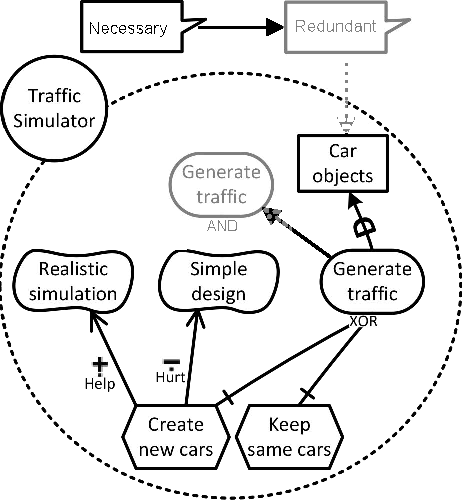
\includegraphics[width=\columnwidth]{img/Example1-new-attack.pdf}
\caption{Example RationalGRL model (extension of Fig.~\ref{fig:example-small2})}
\label{fig:example-small3}
\end{figure} 

We illustrate the new elements using Figure~\ref{fig:example-small3}, which is an extension of Figure~\ref{fig:example-small2}. 

We start with the new element which we call the \emph{Generic Argument}.

\begin{definition}[Generic Argument]
\label{def:generic-argument}
A generic argument $ga \in \mathbb{N}\times Names$ is a relation such that $ga=(id, name)$ means
\begin{itemize}
\item $id\in \mathbb{N}$ is the identifier of the generic argument,
\item $name\in Names$ is a string description of its name.
\end{itemize}
We may refer to the argument with id $i$ simply with $ga_i$. A set of arguments is denoted by $GA$.
\end{definition}

\paragraph{Rationale and example} A generic counterargument is simply an argument that can be used to attack any previous argument, or an IE. It is different from a belief element, since a generic counterargument is used in the computation to determine whether a RationalGRL element is accepted or rejected. Note that one of the constraints of a GRL model (Def.~\ref{def:grl-model}) is that GRL links (Def.~\ref{def:link:contrib},~\ref{def:link:decomp}, and~\ref{def:link:dependency}) should connect IEs, which means that in GRL generic arguments cannot be connected with GRL links. This is correct, since generic arguments are not part of GRL, so they should also not occur in links. 

In Fig.~\ref{fig:example-small3}, there are two generic counterargument which can be formalized as $(19, \text{Redundant})$ and $(20, \text{Necessary})$.

\begin{definition}[Argument]
\label{def:argument}
An argument $A=(elem,type)$ is a pair such that:
\begin{itemize}
\item $elem$ is either an intentional element $ie$ (Def.~\ref{def:ie}), an actor $act$ (Def.~\ref{def:actor}), an Actor-IE relation $r_{ActIE}$ (Def.~\ref{def:act-ie-relation}),  a contribution link $contr$, a decomposition link $decomp$ (Def.~\ref{def:link:decomp}), a dependency link $dep$ (Def.~\ref{def:link:dependency}), or a generic argument $ga$ (Def.~\ref{def:generic-argument}).
\item $type\in Type$ (Def.~\ref{def:set-definitions}) is the type of the argument.
\end{itemize}
\end{definition}

\paragraph{Rationale and example} We define an argument as either a generic argument or any of the GRL elements or links. This captures the specification in the RationalGRL metamodel (Fig.~\ref{fig:metamodel}) in which the class \textsf{Argument} is a superclass of \textsf{GenericArgument} and \textsf{GRLModelElement}, which again is a superclass of both \textsf{ElementLink} and \textsf{GRLLinkableElement}. A \textsf{GRLLinkableElement} is in turn a superclass of \textsf{Actor} and \textsf{IntentionalElement}. In sum, we define an argument simply as any one of the GRL elements or links, or a generic argument.

In Fig.~\ref{fig:example-small3}, the actor, all IEs, all links, and all generic counterarguments are arguments. We will give a full formalization of this after the definition of a RationalGRL model (Def.~\ref{def:rationalgrl-model}).

\begin{definition}[Attack Link]
\label{def:link:attack}
Given a set of arguments $Arg$, an attack link $att\in Arg\times Arg$ is a relation such that $att=(A_i,A_j)$ means:
\begin{itemize}
\item $A_i\in Arg$ is the unique identifier of the element that is performing that attack,
\item $A_j\in Arg$ is the unique identifier of the element that is being attacked.
\end{itemize}
Intuitively, $att=(A_i,A_j)$ means that argument $A_i$ is attacking argument $A_j$. A set of attack links is denoted by $Att$.
\end{definition}

\paragraph{Rationale and example} The attack link is the only link that RationalGRL adds to GRL. In Fig~\ref{fig:example-small3}, there are three attack links. The first two attack links originate from generic counterarguments and involve the following three elements:
\begin{itemize}
\item $A_1 = ((1, Resource, \text{Car objects}, AND), Resource)$
\item $A_{19} = ((19, \text{Necessary}), GenArg)$
\item $A_{20} = ((20, \text{Redundant}), GenArg)$
\end{itemize}

These two attack links are formalized as $(A_{20},A_{19})$ and $(A_{19}, A_1)$.

The third attack link is an attack link created by \emph{replacing} and existing argument (we will discuss this process in more detail in Sect.~\ref{sect:algorithms}). It involves two version of the same IE:
\begin{itemize}
\item $A_{4} = ((5, goal, \text{Generate traffic}, AND), Goal)$
\item $A_{18} = ((5, goal, \text{Generate traffic}, XOR), Goal)$
\end{itemize}

This attack link is formalized at $(A_{18},A_4)$.

The last example shows an important difference between RationalGRL models and valid GRL models: While a valid GRL model disallows multiple elements with the same identifier (Def.~\ref{def:valid-grl-model}, condition 1), RationalGRL models do not enforce this restriction. This is because it is possible to create multiple arguments for the same element, where argument contains different content for the same element. This is what the example above also shows. However, the set of \emph{accepted} elements in a RationalGRL should all have unique identifier (see Def.~\ref{def:valid-rationalgrl-model}).

\begin{definition}[RationalGRL Model]
\label{def:rationalgrl-model}
A \emph{RationalGRL model} $RatGRL=(Arg, Att)$ consists of a set of arguments $Args$ (Def.~\ref{def:argument}) and a set of attack links $Att$ (Def.~\ref{def:link:attack}).
\end{definition}

\paragraph{Rationale and example} The definition of a RationalGRL model collects all the previously defined tuples into a single definition. For completeness, we now provide the full specification of Figure~\ref{fig:example-small3}. Let us first enumerate all the arguments used in this example:
\begin{flalign*}
A_0 = &((0, Actor, \text{Traffic simulator}), Actor)&\\
A_1 = &((1, task, \text{Car objects}, AND), Task),&\\
A_2 = &((2, softgoal, \text{Real. sim.}, AND), Softgoal),&\\
A_3 = &((3, softgoal, \text{Simple des.}, AND), Softgoal),&\\
A_4 = &((4, goal, \text{Generate traffic}, AND), Goal),&\\
A_5 = &((5, task, \text{Create new cars}, AND), Task),&\\
A_6 = &((6, task, \text{Keep same cars}, AND)\}, Task),&\\
A_7 = &((7, 4, 1), Dep),&\\
A_8 = &((8, 5, 2, \text{Help}), Contr),&\\
A_9 = &((9, 5, 3, \text{Hurt}), Contr),&\\
A_{10} = &((10, 5, 4), Decomp),&\\
A_{11} = &((11, 6, 4), Decomp),&\\
A_i = &((0,i-11),ActIE), \text{for } 12\le i\le 17&\\
A_{18} = &((4, goal, \text{Generate traffic}, XOR), Goal),&\\
A_{19} = &((18, \text{Redundant}), GenArg),&\\
A_{20} = &((19, \text{Necessary}), GenArg),&
\end{flalign*}

This model is then formalized as $RationalGRL=(Arg, Att)$ where:
\begin{flalign*}
Arg = &\{A_0,A_1,\ldots,A_{20}\}\\
Att=&\{(A_{18},A_4), (A_{19},A_1), (A_{20},A_{19})\}
\end{flalign*}

All the arguments and the attack relations of this RationalGRL model are shown in Figure~\ref{fig:example-small4}. Note the arguments for Actor-IE containment (arguments $A_{12}$ to $A_{20}$) have been omitted from this figure for readability. It can be read from the figure that two arguments are currently rejected, namely $A_4$ and $A_{19}$. However, we did not yet make precise how exactly this is computed. We will do so in the following definitions.

\begin{figure}[ht]
\centering
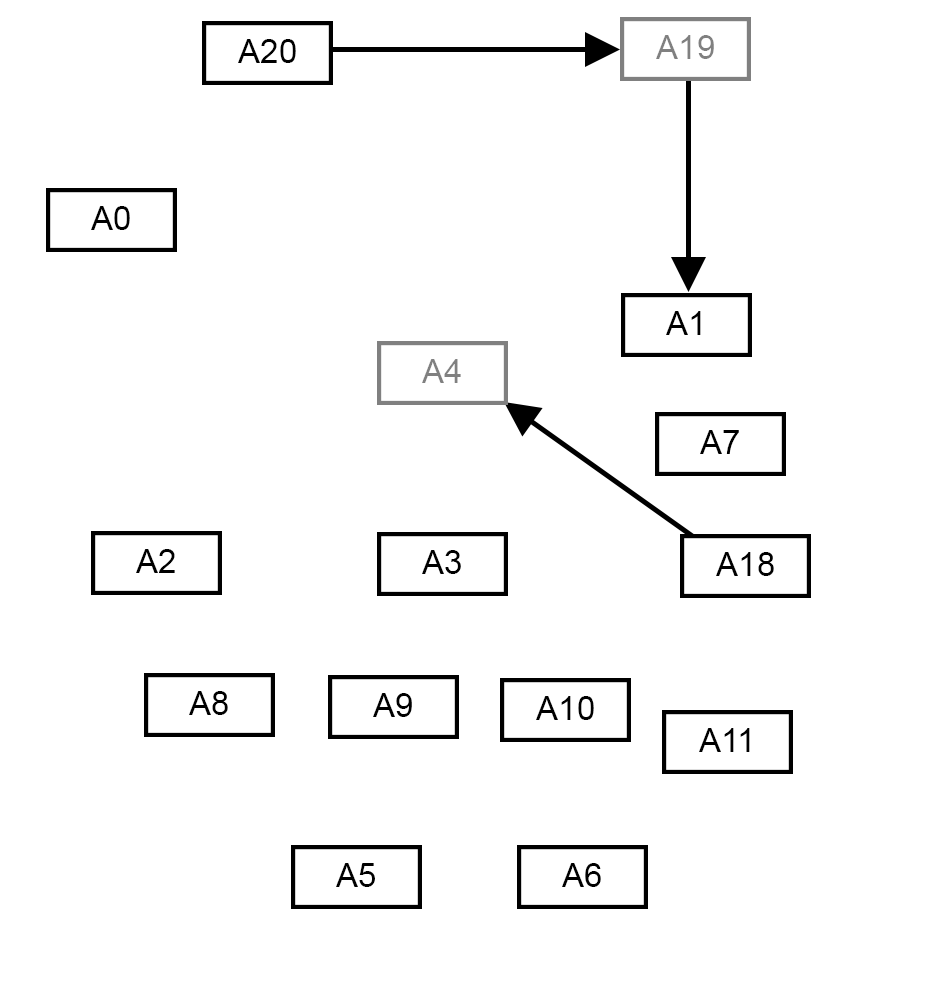
\includegraphics[width=\columnwidth]{img/Example1-new-arguments}
\caption{Argumentation framework of RationalGRL model from Fig.~\ref{fig:example-small3}}
\label{fig:example-small4}
\end{figure} 


In order to compute when an argument is accepted and when not we use argumentation semantics.  We use the standard approach here, which is known as \emph{Dung's semantics}. The following notions are preliminary.

\begin{definition}[Argumentation Framework~\cite{Dung1995}]
\label{def:argumentation-framework}
An \emph{argumentation framework} $AF=(Arg,Att)$ consists of a set of arguments $Arg$ and a set of attack relations $Att\subseteq Arg\times Arg.$
\end{definition}

We see that the definition of an argumentation framework is very close to that of a RationalGRL model. This allows us to use the following results directly.

\begin{definition}[Attack, conflict-freeness, defense, and admissibility~\cite{Dung1995}] Suppose an argumentation framework $AF=(Arg,Att)$, two sets of arguments $S\cup S'\subseteq Arg$, and some argument $A\in Arg$. We say that
\begin{itemize}
\item $S$ \emph{attacks} $A$ if some argument in $S$ attacks $A$,
\item $S$ \emph{attacks} $S'$ if some argument in $S$ attacks some argument in $S'$,
\item $S$ is \emph{conflict-free} if it does not attack itself,
\item $S$ \emph{defends} $A$ if for each $B$ such that $B$ attacks $A$, $S$ attacks $B$,
\item $S$ is \emph{admissible} if $S$ is conflict-free and defends each argument in it.
\end{itemize}
\end{definition}

\begin{figure}[ht!]
\centering
\begin{tikzpicture}
        \node[minimum size=1cm] (a20) [argNodeIN] at (-3,0) {$A_{20}$};
        \node[minimum size=1cm] (a19) [argNodeIN] at (0,0) {$A_{19}$};
        \node[minimum size=1cm] (a1) [argNodeIN] at (3,0) {$A_1$};
             
         \path
    (a20) edge [attackLink] (a19)
    (a19) edge [attackLink] (a1);
    
\end{tikzpicture}
\caption{Example argumentation framework, subset of Fig.~\ref{fig:example-small4}.}
\label{fig:goalmodeling:arg2}
\end{figure}

Let us explain these definitions using the example argumentation framework in Figure~\ref{fig:goalmodeling:arg2}, which is a subset of Figure~\ref{fig:example-small4} containing only arguments $A_1, A_{19}$, and $A_{20}$. In this example, there are two admissible sets: $\{A_{20}\}$ and $\{A_1, A_{20}\}$. In the last admissible set, $A_{20}$ defends $A_1$ against its attacker $A_{19}$. Sets containing both $A_{19}$ and either $A_1$ or $A_{20}$ are not conflict free, and the sets $\{A_1\}$ and $\{A_{19}\}$ do not defend themselves against $A_{19}$ and $A_{20}$, respectively. 

Given the notion of admissible sets, we can then define our argumentation semantics. There are a large number of different semantics to determine which arguments are acceptable; in this article, we focused on the preferred semantics.

\begin{definition}[Preferred semantics~\cite{Dung1995}] 
\label{def:preferred-semantics}
A preferred extension of an argumentation framework $(Arg,Att)$ is a maximal (w.r.t. set inclusion) admissible set of $R$.
\end{definition}

In our example from Figure~\ref{fig:goalmodeling:arg2}, there is one preferred extension, namely $\{A_{20},A_1\}$. Returning to our running example of Figure~\ref{fig:example-small3}, this means that the intentional elements \text{Car objects} (task) and the generic counerargument \emph{Necessary} are both \emph{accepted}, while the generic counter argument ``Redundant'' is rejected.

\subsection{Translation algorithms}

Now that we have formalized both a GRL model and a RationalGRL model, we develop algorithm in order to translate between these two models. Both of these two translation algorithms are straightforward. Their main task is to ensure that in RationalGRL models, the GRL elements and links are wrapped in an argument with the corresponding type.

\paragraph{GRL to RationalGRL Translation} We start with the translation algorithm from GRL to RationalGRL, which is shown in Algorithm~\ref{alg:translation:to-rationalgrl}.  The translation algorithm translates all of the GRL elements and links into arguments. It takes a GRL model as input. Recall that a GRL model is defined as $GRL=(IE, Bel, Act, R_{ActIE}, Bellink, Contr, Decomp, Dep)$ (Def.~\ref{def:grl-model}). Then, on line~\ref{alg:translation:to-rationalgrl:init}, the set of arguments is initialized with the empty set. Each of the five for loops in the algorithm translates a different GRL component into an argument. For instance, in the for loop starting at line~\ref{alg:translation:to-rationalgrl:ie}, all IEs are added as pairs consisting of the IE itself, and its corresponding type. This is in line with the definition of an argument~\ref{def:argument}). Since the other for loops are very similar, we do not explain them here. At line~\ref{alg:translation:to-rationalgrl:return}, the algorithm returns a RationalGRL model $(Arg,\emptyset)$ containing all arguments in $Arg$, and an empty set of attack relations. 

\begin{algorithm}[h]
  \caption{GRL to RationalGRL Translation}
  \label{alg:translation:to-rationalgrl}
  \begin{algorithmic}[1]
    \Procedure{$TranslateToRationalGRL$}{$GRL$}
    \State $Arg \leftarrow \emptyset$\label{alg:translation:to-rationalgrl:init}
    \For{$ie\in IE$}\label{alg:translation:to-rationalgrl:ie}
      \State $Arg \leftarrow Arg \cup \{(ie,ie.type)\}$
    \EndFor
    \For{$act\in Act$}
      \State $Arg \leftarrow Arg \cup \{(act, Actor)\}$
    \EndFor
    \For{$actIE\in ActIE$}
      \State $Arg \leftarrow Arg \cup \{(actIE, ActIE)\}$
    \EndFor
    \For{$contr\in Contr$}
      \State $Arg \leftarrow Arg \cup \{(contr, Contr)\}$
    \EndFor
    \For{$dep\in Dep$}
      \State $Arg \leftarrow Arg \cup \{(dep, Dep)\}$
    \EndFor
    \For{$decomp\in Decomp$}
      \State $Arg \leftarrow Arg \cup \{(decomp, Decomp)\}$
    \EndFor
    \State \Return $(Arg, \emptyset)$\label{alg:translation:to-rationalgrl:return}
    \EndProcedure
  \end{algorithmic}
\end{algorithm}

\paragraph{RationalGRL to GRL translation} The translation from a RationalGRL model to a GRL model is given in Algorithm~\ref{alg:translation:to-grl}. It is very similar to the previous algorithm, but then works in the other direction. In this case, arguments are unpacked and put in the corresponding IE components. The most important difference between the previous algorithm and this one is that in the RationalGRL to GRL translation, argumentation semantics is used to determine the \emph{preferred extension} (Def.~\ref{def:preferred-semantics}). This is a set containing all accepted arguments. The GRL is then generated from all the accepted arguments. This is done by iterating over all arguments in the extension in line~\ref{alg:translation:to-grl:extension-iter}. The switch statement on line~\ref{alg:translation:to-grl:switch} then does a case distinction on the type of the arguments, and each case ensures the argument is put in the right GRL component. Finally, the algorithm returns a GRL model on line~\ref{alg:translation:to-grl:return}.

\begin{algorithm}[h]
  \caption{RationalGRL to GRL Translation}
  \label{alg:translation:to-grl}
  \begin{algorithmic}[1]
    \Procedure{$TranslateToGRL$}{$RatGRL$}
    \State $E \leftarrow ComputeExtension(Arg,Att)$
    \State $IE\leftarrow\emptyset$, $Act\leftarrow\emptyset$, $R_{ActIE}\leftarrow\emptyset$, $Contr\leftarrow\emptyset$
    \State $Decomp\leftarrow\emptyset$, $Dep\leftarrow\emptyset$
    \For{$(Elem, T)\in E$}\label{alg:translation:to-grl:extension-iter}
      \Switch{$T$}\label{alg:translation:to-grl:switch}
          \Case{$T\in Type$}
            \State $IE\leftarrow IE\cup \{Elem\}$
          \EndCase
          \Case{$T = Actor$}
            \State $Act\leftarrow Act \cup\{Elem\}$
          \EndCase
          \Case{$T=Contr$}
            \State $Contr\leftarrow Contr\cup \{Elem\}$
          \EndCase
          \Case{$T=Dep$}
            \State $Dep\leftarrow Dep\cup \{Elem\}$
          \EndCase
          \Case{$T=Decomp$}
            \State $Decomp\leftarrow Decomp\cup\{Elem\}$
          \EndCase
      \EndSwitch
    \EndFor
    \State \Return $(IE,Act,R_{ActIE}, Contr, Decomp, Dep)$\label{alg:translation:to-grl:return}
    \EndProcedure
  \end{algorithmic}
\end{algorithm}

\paragraph{Valid RationalGRL model} While we have defined a notion of a \emph{valid GRL model} (Def.~\ref{def:valid-grl-model}), we have not done so for a RationalGRL model yet. This is because it depends on the translation procedure. We define a RationalGRL model as valid if and only if the RationalGRL to GRL translation results in a valid GRL model. In this way, we do not have to reiterate all conditions on a GRL model, but use the translation algorithm.

\begin{definition}[Valid RationalGRL Model]
\label{def:valid-rationalgrl-model}
A RationalGRL model $RatGRL = (Arg, Att)$ with preferred extension $E=(A_1,\ldots,A_n)$ is a \emph{valid RationalGRL model} iff $TranslateToGRL(RatGRL)$ (Alg.~\ref{alg:translation:to-grl}) is a valid GRL model (Def.~\ref{def:valid-grl-model}).
\end{definition}

\subsection{Algorithms for argument schemes and critical questions}
\label{sect:algorithms}

In the previous section we formalized a \emph{static} representation of the RationalGRL framework. In this section we formalize the \emph{dynamics}. We do so by developing algorithms for applying argument schemes and critical questions in the context of a RationalGRL model (Def.~\ref{def:rationalgrl-model}). These algorithms produce new elements and attack relations. We can then use argumentation semantics (Def.~\ref{def:semantics}) to compute sets of accepted arguments. The content of these arguments is then used to compute the resulting RationalGRL model, together with enabled and disabled GRL elements and their underlying arguments.

\paragraph{Argument Schemes}

In all of the following algorithms, we assume the following
\begin{itemize}
\item There algorithms are being applied to some valid RationalGRL model $RatGRL$,
\item The procedure $mindId()$ generates a new unique id.
\end{itemize}

The algorithms for applying argument schemes are short, and consist simply of adding an argument for the element that is being added.

\begin{algorithm}[h]
  \caption{AS0: Add a new actor with name $n$}\label{alg:as0}
  \begin{algorithmic}[1]
    \Procedure{$AS_0$}{$n$}
    \State $actor \leftarrow (mintId(), n)$ \label{alg:as0:1}
    \State $Arg\leftarrow Arg \cup \{(actor,Actor)\}$\label{alg:as0:2}
    \EndProcedure
  \end{algorithmic}
\end{algorithm}

\paragraph{Rationale and example} The algorithm takes one argument, namely the name of the actor $n$. On line~\ref{alg:as0:1} of the algorithm, a new (unique) id is minted as the identifier of the new actor, which is assigned with its corresponding name to the variable $actor$. On line~\ref{alg:as0:2} the pair $(actor,Actor)$ is added as a new argument, indicating that an argument of type $Actor$ is added.

\begin{algorithm}[h]
  \caption{Applying AS1: Actor with id $i$ has resource $n$}\label{alg:as1}
  \begin{algorithmic}[1]
    \Procedure{$AS_1$}{$i, n$}
    \State $rId\gets mintId()$
    \State $r\leftarrow (rId, Resource, n, AND)$
    \State $Arg\gets Arg\cup \{(r, Resource),(i,rId)\}$
    \EndProcedure
  \end{algorithmic}
\end{algorithm}

\paragraph{Rationale and example} Explain here...

\begin{algorithm}[h]
  \caption{Applying AS5: Goal with id $i$ decomposes into tasks $t$}\label{alg:as5}
  \begin{algorithmic}[1]
    \Procedure{$AS_5$}{$i, t$}
    \State $tId\gets mintId()$
    \State $t\leftarrow (tId, Task, t, AND)$
    \State $Arg\gets Arg\cup \{(t, Task),(i,tId)\}$
    \EndProcedure
  \end{algorithmic}
\end{algorithm}

\paragraph{Rationale and example} Explain here.


The remaining argument schemes are all very similar, in the sense that they all simply add a single argument to the set of arguments containing the element to be added. We therefore have omitted them here.

\subsubsection*{Algorithms for critical questions}

We now develop algorithms for our critical questions. Recall that answering a critical question can have four effects, and we discuss each of these effects separately.

\begin{algorithm}[h]
  \caption{Applying DISABLE: Element $i$ is disabled}\label{alg:disable}
  \begin{algorithmic}[1]
    \Procedure{DISABLE}{$i$}
    \State $id\gets id+1$
    \State $A\gets \{disabled(i))\}$
    \State $Args \gets Args\cup A$
    \EndProcedure
  \end{algorithmic}
\end{algorithm}

\todo{Marc}{Marc}{Here we would add an argument and an attack from the argument to the intentional element. We don't add ``disabled'' because this is what argumentation semantics should do for us.}

\emph{Algorithm~\ref{alg:disable} (\textsf{DISABLE}) for critical questions CQ0-CQ5a, CQ6a, CQ7a, CQ8, CQ11, and CQ12:} The disable operation consists of adding an argument stating the GRL element with identifier $i$ is disabled. Let us reconsider the example of Figure~\ref{fig:examples:relevant-actor}. This example consists of an instantiation of argument scheme AS0, which is attacked by an argument that resulted from answering critical question. The instantiation of AS0 leads to the argument $A=\{actor(0),name(0,dev\_team\}$. After applying $DISABLE(0)$ we obtain the arguments: $$Args=\{\{actor(0),name(0,dev\_team\}, \{disabled(0)\}\}.$$ Note that our implementation of this attack does not lead to an actual attack in the argumentation framework.

\begin{algorithm}[h]
  \caption{Answering CQ5b: ``Does goal $G$ decompose into any other tasks?'' With: ``Yes, namey into tasks $t_1,\ldots,t_k$''}\label{alg:cq5b}
  \begin{algorithmic}[1]
    \Procedure{CQ5b}{$g_{id},\{i_1,\ldots,i_n\}, type, \{t_1,\ldots,t_k\}$}
    \State $T_{id} = \{i_1,\ldots,i_n\}$
    \For{$t_i$ in $\{t_1,\ldots,t_k\}$}\label{alg:cq5b:for1}
      \If{$\exists_{A\in Args} \{task(t_{id}),name(t_{id},t_i)\}\subseteq A$}
        \State $T_{id} \gets T_{id} \cup \{t_{id}\}$
      \Else
        \State $id\gets id+1$
        \State $A \gets \{task(id),name(id,t_i)\}$
        \State $Args \gets Args\cup A$
        \State $T_{id} \gets T_{id} \cup \{id\}$
      \EndIf
    \EndFor
    \State $id\gets id+1$
    \State $A_{new} = \{decomp(id, g_{id}, T_{id}, type)\}$\label{alg:cq5b:newarg}
    \For{$A$ in $\{decomp(\_,g_{id},\_,\_)\}\subseteq A\mid A\in Args\}$}\label{alg:cq5b:for2}
      \State $Att\gets Att \cup \{(A_{new},A)\}$
    \EndFor
    \State $Args \gets Args \cup \{A_{new}\}$
    \EndProcedure
  \end{algorithmic}
\end{algorithm}

\emph{Algorithm~\ref{alg:cq5b} (\textsf{REPLACE}) for critical questions CQ5b:} This algorithm is executed when critical question CQ5b is answered, which is a critical question for argument scheme AS5. Therefore, it assumes an argument for a goal decomposition already exists of the following form (see Algorithm~\ref{alg:as5}): $$\{decomp(d, g_{id}, \{i_1,\ldots,i_n\},type).$$  The goal of the algorithm is to generate a new argument of the form $decomp(d, g_{id}, \{i_1,\ldots,i_5\}\cup \{j_1,\ldots,j_k\}, type)$, where $\{j_1,\ldots,j_k\}$ are the identifiers of the additional decomposing tasks $\{t_1,\ldots,t_k\}$.

The algorithm takes as input the goal identifier $g_{id}$, the set of existing decomposing task identifiers $i_1,\ldots,i_n$, the decomposition type, and the names of the new tasks $t_1,\ldots,t_k$ that should be added to the decomposition. The first part of the algorithm is familiar from Algorithm~\ref{alg:as5}: For each task name we check whether it already exists as an argument (line 4), and if it doesn't (line 6) we add a new argument for it. After the for-loop (line 13), a new argument is created for the new decomposition relation (14). After this, the for-loop on line 15 ensures that the new argument attacks all previous arguments for this decomposition (note that the variable ``$\_$'' means ``do not care''). Only at the very end the new argument is added (line 18), to ensure it does not attack itself after the for loop of line 15-17. 

An example of this algorithm is shown in Figure~\ref{fig:examples:cq5b}.\footnote{Note that part of the arguments (the statements about actors) have been omitted from the figure for readability.} Before the critical question is applied, the following arguments have been put forward:
\begin{itemize}
\item $\{goal(0),name(0,show\_simulation)\}$
\item $\{task(1),name(1,generate\_traffic)\}$
\item $\{task(2),name(2,compute\_lights)\}$
\item $\{decomp(3,0,\{1,2\},and)\}$.
\end{itemize}

Next, Algorithm~\ref{alg:cq5b} is called as follows: $CQ5b(0,\{1,2\},and,\{show\_controls\})$. That is, the existing decomposition is challenged by stating that goal $show\_simulation$ not only decomposes into $generate\_traffic$ and $compute\_lights$, but it also decomposes into $show\_controls$. Since this task does not exist yet, it is created by the algorithm, which also ensures the new argument for the decomposition link attacks the previous argument for the decomposition link.

\begin{figure*}[ht!]
\centering
        \begin{tikzpicture}
        \node (a0) [argNodeIN,minimum width=1.5cm] at (-5,0) {
        	\smallargtext{AS3}{$\{goal(0),$\\$name(0,show\_sim\}$}
        };
        \node (a1) [argNodeIN] at (0,0) {
        \smallargtext{AS2}{$\{task(1),$\\$name(1,gen\_traffic\}$}
        };
        \node (a2) [argNodeIN] at (5,0) {
        \smallargtext{AS2}{$\{task(3),$\\$name(2,show\_ctrls\}$}
        };
        \node (a2a) [argNodeIN] at (-2.5,-2) {
        \smallargtext{AS2}{$\{task(2),$\\$name(2,comp\_lights\}$}
        };
        \node (a3) [argNodeOUT] at (-3,-4) {$\{decomp(3,0,\{1,2\},and\}$
        };
        \node (a4) [argNodeIN] at (3,-4) {$\{decomp(3,0,\{1,2,3\},and\}$
        };
         
         \path
    (a4) edge [attackLink] (a3)
    (a3) edge [CQLink, bend right=50] node [below,draw=none] {CQ5b} (a4)
    (a4) edge [CQLink] node [left,draw=none] {CQ5b} (a2);
\end{tikzpicture}
\caption{Example of applying critical question CQ5b (Algorithm~\ref{alg:cq5b})}
\label{fig:examples:cq5b}
\end{figure*}

\emph{Algorithms for critical questions CQ10a and CQ10b (REPLACE)}: These algorithms have a very similar structure as Algorithm~\ref{alg:cq5b} and have therefore been omitted.

\begin{algorithm}[h]
  \caption{Answering CQ13: ``Is the name of element $i$ clear?'' With: ``No, it should be $n$''}\label{alg:cq13}
  \begin{algorithmic}[1]
    \Procedure{CQ13}{$i, n$}
    \State $ArgsN \gets\{ A\in Args \mid name(i,x)\in A\}$
    \State $B\gets B'\backslash \{name(i,\_)\}$ with $B'\in ArgsN$
    \State $A \gets B \cup \{name(i,n)\}$
    \State $Args \gets Args \cup \{A\}$
    \For{$C$ in $ArgsN$}
      \State $Att\gets Att \cup \{(A,C)\}$
    \EndFor
    \EndProcedure
  \end{algorithmic}
\end{algorithm}

\emph{Algorithms for critical question CQ13 (REPLACE):} This algorithm is used to clarify/change the name of an element. It takes two parameters: the element identifier $i$ and the new name $n$. The idea behind the algorithm is that we construct a new argument for $n$, and to ensure that this argument attacks all previous arguments for giving a name to this element. Here we can use the following fact: Suppose $Args$ is a set of arguments, each containing an atom about the name for an element $i$, i.e. for all $A\in Args: name(i,_)\in Args$, then all arguments in $Args$ are the same except for the $name$ atoms, i.e. for all $A,B\in Args: A\backslash\{name(i,_)\} = B\backslash\{name(i,_)\}$. This means that if we would like to attack every argument of $Args$ with a new argument that replaces the $name$ atom, we can simply take any argument in $Args$, remove the previous $name$ atom, add the new one and attack all arguments in $Args$. This is exactly what the algorithm does.


On line 2, all arguments that have been put forward for this element and contain $name(i,x)$ are collected into the set $ArgsN$. On line 3, some arguments $B'\in ArgsN$ minus the $name$ statement is assigned to $B$ (note that it does not matter which one we pick), and on line 4 $B$ is joined with the new $name$ statement and stored in $A$, which is then added to the set of arguments $Args$. The for-loop on lines 6-8 ensures all previous arguments for names of the element are attacked by the new argument.

\begin{figure}[ht!]
\centering
        \begin{tikzpicture}[->]
        \node (a0a) [argNodeIN] at (-2,2) {
        	\longargtext{AS0}{$\{actor(0),name(0,student)\}$}
        };
        \node (a0) [argNodeOUT] at (-2,0) {
        	\longargtext{AS2}{$\{task(1),name(1,create\_road),has(0,1)\}$}
        };
        \node (a1) [argNodeOUT] at (-2,-2) {
        	\longargtext{AS2}{$\{task(1),name(1,choose\_pattern),has(0,1)\}$}
        };
        \node (a2) [argNodeOUT] at (-2,-4) {
        	\longargtext{AS2}{$\{task(1),name(1,pattern\_pref),has(0,1)\}$}
        };
        \node (a3) [argNodeIN] at (-2,-6) {
        	\longargtext{AS2}{$\{task(1),name(1,road\_pattern),has(0,1)\}$}
        };
\begin{pgfonlayer}{background}
         \path
    (a1) edge[attackLink] (a0)
    (a2) edge[attackLink] (a1)
    (a2) edge[attackLink, bend right=20] (a0)
    (a3) edge[attackLink] (a2)
    (a3) edge[attackLink, bend right=20] (a1)
    (a3) edge[attackLink, bend right=40] (a0);
\end{pgfonlayer}

	\path
	(a0) edge [CQLink, bend right=50] node [left,draw=none] {CQ13} (a1)
    (a1) edge [CQLink, bend right=50] node [left,draw=none] {CQ13} (a2)
    (a2) edge [CQLink, bend right=50] node [left,draw=none] {CQ13} (a3);
\end{tikzpicture}
\caption{Applying critical question CQ13 (Algorithm~\ref{alg:cq13}) to the example in Figure~\ref{fig:examples:clarification}.}
\label{fig:examples:clarification:formal}
\end{figure} 

An example of of Algorithm~\ref{alg:cq13} is shown in Figure~\ref{fig:examples:clarification:formal}. Let us consider the last application of CQ13 (bottom argument). Before this application, the following arguments have been put forward:
\begin{itemize}
\item $A_1$: $\{actor(0),name(0,student)\}$
\item $A_2$:$\{task(1),name(1,create\_road),has(0,1)\}$
\item $A_3$ $\{task(1),name(1,choose\_pattern),has(0,1)\}$
\item $A_4$:$\{task(1),name(1,pattern\_pref),has(0,1)\}$
\end{itemize}
The algorithm is now called as follows: $CQ13(1,road\_pattern)$, i.e., the new name of the element should be $road\_pattern$. Let us briefly run through the algorithm. After executing line 2 we obtain $ArgsN=\{A_2,A_3,A_4\}$, since only those arguments contain $name(1,\_)$. Next, on line 3, $B=\{task(1),has(0,1)\}$, i.e., $B$ is the general argument for the task without the $name$ statement. After line 4 we have $$A=\{task(1),has(0,1),name(1,road\_pattern),$$ which is added to $Args$ and attacks arguments $A_2,A_3$, and $A_4$. 

\emph{Algorithms for critical questions CQ6b, CQ6c, CQ6d, CQ7b, and CQ9 (INTRO):} The introduction algorithms for the critical questions are all very similar to the INTRO algorithms for argument schemes (Algorithm~\ref{alg:as1}). They have therefore been omitted.

\begin{algorithm}[h]
  \caption{Generic counterargument to argument $A$}\label{alg:cq6b}
  \begin{algorithmic}[1]
    \Procedure{Attack}{$A$}
    \State $A_{new} = \{\}$
    \State $Args \gets Args \cup \{A_{new}\}$
    \State $Att \gets Att \cup \{(A_{new},A)\}$
    \EndProcedure
  \end{algorithmic}
\end{algorithm}

\emph{Algorithm for $Att$ (Generic counter argument:} Applying a generic counter argument is very simple, and simply results on an attack on the original argument. We illustrate this by continuing our example from Figure~\ref{fig:examples:relevant-actor2:formal} (Algorithm~\ref{alg:as0}). The example is shown in Figure~\ref{fig:examples:relevant-actor2:formal}, where we see that a generic counter argument simply attacks the argument to disable the actor.

\begin{figure}[ht!]
\centering
        \begin{tikzpicture}
        \node (a0) [argNodeIN] at (-3.7,0) {
        	\smallargtext{AS0}{$\{actor(0),name(0,dev\_team\}$}
        } ;
        \node (a1) [argNodeOUT] at (-3.7,-2){
        	\argtext{DISABLE}{$\{disabled(0)\}$}
        };
        \node (a2) [argNodeIN] at (-3.7,-4){
        	\argtext{Att}{$\{\}$}
        };
         \path
    (a0) edge [CQLink, bend right=50] node [left,draw=none] {CQ0} (a1)
    (a1) edge [CQLink, bend right=50] node [left,draw=none] {Att} (a2)
    (a2) edge [attackLink] (a1);
\end{tikzpicture}
\caption{Formalization of the arguments in Figure~\ref{fig:examples:relevant-actor2}.}
\label{fig:examples:relevant-actor2:formal}
\end{figure}

\subsection{Constructing GRL models}
\label{sect:rationalGRL-GRL}
\todo{F}{F,M}{Dit is snel getypt, moet nog checken of het klopt.}

\begin{definition}[RationalGRL model] A RationalGRL model $\mathcal{R}$ is an argumentation framework $AF=(Args,Att)$ where all arguments in $Args$ and attacks in $Att$ are based on algorithm X-XX.  
\end{definition}

\begin{definition}[GRL model] A GRL model $\mathcal{M}$ based on a RationalGRL model $\mathcal{R}$ is the preferred extension of $\mathcal{R}$.  
\end{definition}
=======
\todo{F}{F,M}{It would be good to have a formal definition of how to construct models given an argumentation framework. If we define a model M at the start of this section, this should be fairly easy.}

Constructing GRL models from the arguments is extremely simple: We simply compute the extensions of the argumentation frameworks, and collect all atomic sentences in the accepted arguments. This forms out GRL model. Let us briefly do so for the examples of the previous subsection:
\begin{itemize}
\item
Figure~\ref{fig:examples:relevant-actor:formal}: Since there are no attacks between the arguments, all atomic sentences are accepted. This results in the following specification: 
\begin{quote}
\begin{verbatim}
actor(0).
name(0,dev_team).
disabled(0).
\end{verbatim}
\end{quote}
This again corresponds to the GRL model on the right-hand side of Figure~\ref{fig:examples:relevant-actor}.
\item
Figure~\ref{fig:examples:cq5b}: There is one rejected argument and five accepted ones. The resulting specification is:
\begin{quote}
\begin{verbatim}
goal(0). name(0,show_simulation).
task(1). name(1,generate_traffic).
task(2). name(2,compute_lights).
task(3). name(3,show_controls).
decomp(3,0,{1,2,3},and).
\end{verbatim}
\end{quote}
\item Figure~\ref{fig:examples:clarification:formal}: There are only two accepted arguments. The resulting specification is:
\begin{quote}
\begin{verbatim}
actor(0). name(0, student).
task(1).  name(1,road_pattern).
has(0,1).
\end{verbatim}
\end{quote}
This corresponds to the right-hand GRL model of Figure~\ref{fig:examples:clarification}.
\item Figure~\ref{fig:examples:relevant-actor2:formal}. There are two accepted arguments, but the \emph{generic counterargument} does not contain any formulas. Therefore the resulting specification is:
\begin{quote}
\begin{verbatim}
actor(0).
name(0,dev_team).
\end{verbatim}
\end{quote}
This corresponds to the right-hand GRL model of Figure~\ref{fig:examples:relevant-actor2}.
\end{itemize}